\documentclass{book}
\usepackage[spanish]{babel}
\usepackage[T1]{fontenc}
\usepackage[utf8]{inputenc}
\usepackage{amsmath, amssymb}
\usepackage{dsfont}
\usepackage{graphics}
\usepackage{cases}
\usepackage{graphicx}
\usepackage{pgf}
\usepackage{epsfig}
\usepackage{amssymb}
\usepackage{multirow}
\usepackage{amstext}
\usepackage[ruled,vlined,lined]{algorithm2e}
\usepackage{listings}
\usepackage{amsmath}
\usepackage{epic}
\usepackage{epsfig}
\usepackage{fontenc}
\usepackage{framed,color}
\usepackage{palatino, url, multicol}



\begin{document}

\chapter{Procesamiento del Lenguaje Natural}

El volumen de datos textuales digitalizados que se genera cada día es enorme (por ejemplo, la web, redes sociales, registros médicos, libros digitalizados). Por lo tanto, también crece la necesidad de traducir, analizar y gestionar esta avalancha de palabras y texto.

El procesamiento del lenguaje natural (PLN) es el campo que se encarga de diseñar métodos y algoritmos que toman como entrada o producen como salida datos de \textbf{lenguaje natural} no estructurado \cite{goldberg2017neural}. El PLN se centra en el diseño y análisis de algoritmos computacionales y representaciones para procesar el lenguaje humano \cite{jacobbook}.



Una tarea común de PLN es el Reconocimiento de Entidades Nombradas (NER, por sus siglas en inglés). Por ejemplo:

\begin{figure}[h]
	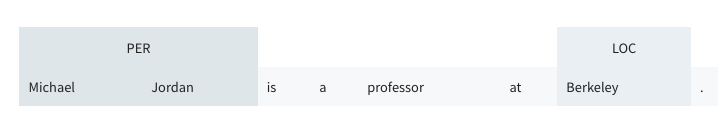
\includegraphics[scale=0.4]{pics/NER.png}
	\caption{Reconocimiento de Entidades Nombradas}
\end{figure}

El lenguaje humano es altamente ambiguo, como en las frases: "Comí pizza con amigos", "Comí pizza con aceitunas" o "Comí pizza con un tenedor". Además, el lenguaje está en constante cambio y evolución, como ocurre con los hashtags en Twitter.

\section{PLN y Lingüística Computacional}

El procesamiento del lenguaje natural (PLN) desarrolla métodos para resolver problemas prácticos relacionados con el lenguaje \cite{JohnsonMLSS}.

Algunos ejemplos son:

\begin{itemize}
  \item Reconocimiento automático del habla.
  \item Traducción automática.
  \item Extracción de información de documentos.
\end{itemize}

La lingüística computacional (LC) estudia los procesos computacionales subyacentes al lenguaje (humano).

\begin{itemize}
  \item ¿Cómo comprendemos el lenguaje?
  \item ¿Cómo producimos el lenguaje?
  \item ¿Cómo aprendemos el lenguaje?
\end{itemize}

El PLN y la LC utilizan métodos y modelos similares.


Aunque existe una superposición sustancial, hay una diferencia importante en el enfoque. La LC se centra en la lingüística respaldada por métodos computacionales (similar a la biología computacional o la astronomía computacional). En lingüística, el lenguaje es el objeto de estudio. El PLN se centra en resolver tareas bien definidas relacionadas con el lenguaje humano (como la traducción, la respuesta a consultas, las conversaciones). Si bien los conocimientos lingüísticos fundamentales pueden ser cruciales para realizar estas tareas, el éxito se mide en función de si y cómo se logra el objetivo (según una métrica de evaluación) \cite{jacobbook}.



El procesamiento del lenguaje natural y la lingüística computacional están estrechamente relacionados y se superponen en muchos aspectos. Ambos campos utilizan métodos y modelos similares para abordar problemas relacionados con el lenguaje humano. Sin embargo, la diferencia principal radica en el enfoque: la lingüística computacional se centra en la lingüística respaldada por métodos computacionales, mientras que el procesamiento del lenguaje natural se centra en resolver tareas prácticas relacionadas con el lenguaje. Ambos campos son fundamentales para comprender y aprovechar el poder del lenguaje humano en la era digital.


\section{Niveles de descripción lingüística}

El campo de la \textbf{descripción lingüística} abarca diferentes niveles:

\begin{itemize}
  \item \textbf{Fonética y fonología:} estudio de los sonidos del habla.
  \item \textbf{Morfología:} estudio de la estructura de las palabras.
  \item \textbf{Sintaxis:} estudio de la estructura de las oraciones.
  \item \textbf{Semántica:} estudio del significado de las palabras y oraciones.
  \item \textbf{Pragmática:} estudio del uso del lenguaje en el contexto.
\end{itemize}

El PLN puede abordar tareas en cada uno de estos niveles, pero a menudo se enfoca en niveles más altos de representación y comprensión.




\subsection{Fonética}

La fonética es la rama de la lingüística que se ocupa del estudio de los sonidos del lenguaje. Examina los órganos utilizados en la producción de sonidos, como la boca, la lengua, la garganta, la nariz, los labios y el paladar. Los sonidos del lenguaje se dividen en vocales y consonantes. Las vocales se producen con poca restricción del flujo de aire desde los pulmones, mientras que las consonantes implican alguna restricción o cierre en el tracto vocal \cite{JohnsonMLSS, fromkin2018introduction}. Además, el Alfabeto Fonético Internacional (AFI) proporciona una notación alfabética para representar los sonidos fonéticos.

\subsection{Fonología}

La fonología se centra en el estudio de cómo los sonidos del habla forman patrones y construyen significado. Los fonemas son las unidades básicas de sonido que diferencian el significado de las palabras. Por ejemplo, en inglés, la "p" y la "b" son fonemas distintos porque cambian el significado de las palabras en las que se encuentran. La fonología también examina las variaciones en la pronunciación de los sonidos en diferentes contextos y dialectos \cite{fromkin2018introduction}.

\subsection{Morfología}

La morfología se ocupa del estudio de la estructura interna de las palabras. Los morfemas son las unidades mínimas de significado que componen las palabras. Por ejemplo, en la palabra "deshacer", los morfemas son "des-", "hacer" y "-er". La morfología también se interesa por los procesos de formación de palabras, como la derivación, donde se agregan prefijos o sufijos a una palabra existente para formar una nueva palabra con un significado diferente \cite{JohnsonMLSS}.

\begin{itemize}
\item Morphology studies the structure of words (e.g.,re+structur+ing, un+remark+able) \cite{JohnsonMLSS}
\item Morpheme: The linguistic term for the most elemental unit of grammatical form \cite{fromkin2018introduction}. Example morphology= morph + ology (the science of).
\item Derivational morphology: process of forming a new word from an existing word, often by adding a prefix or suffix
\item Derivational morphology exhibits a hierarchical structure. Example: re+vital+ize+ation
     \begin{figure}[h]
        	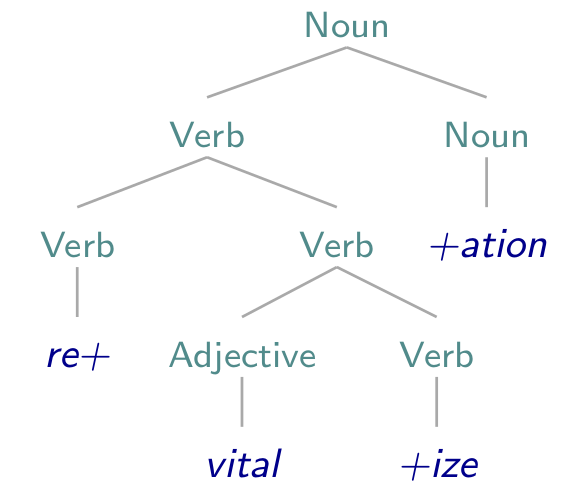
\includegraphics[scale = 0.2]{pics/morphology.png}
        \end{figure}
\item The suffix usually determines the syntactic category (part-of-speech) of the derived word.
\end{itemize}

\subsection{Sintaxis}

La sintaxis es el estudio de cómo las palabras se combinan para formar frases y oraciones gramaticales. Examina las reglas y estructuras que determinan la organización de las palabras en una oración y cómo influyen en el significado. La sintaxis también se ocupa de la relación entre las palabras y las funciones que desempeñan dentro de una oración. Por ejemplo, en la oración "El perro persigue al gato", "el perro" es el sujeto, "persigue" es el verbo y "al gato" es el complemento directo \cite{JohnsonMLSS}.

\begin{itemize}
\item Syntax studies the ways words combine to form phrases and sentences \cite{JohnsonMLSS}
     \begin{figure}[h]
        	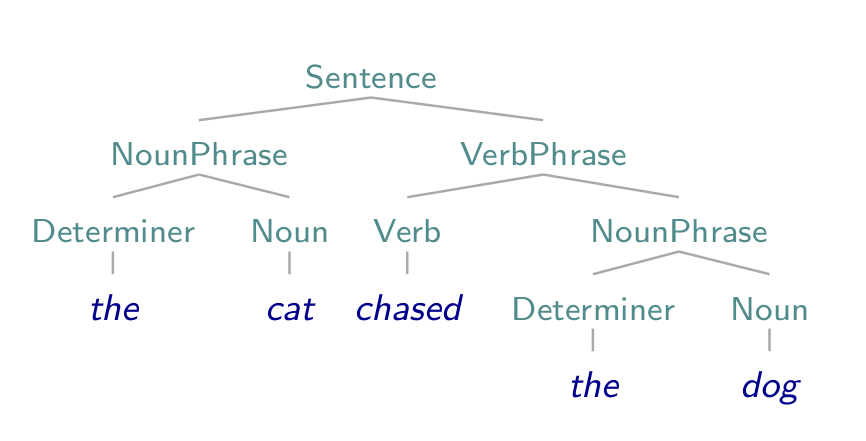
\includegraphics[scale = 0.3]{pics/parseTree1.png}
        \end{figure}
\item Syntactic parsing helps identify \textbf{who did what to whom}, a key step in
understanding a sentence.
\end{itemize}


\subsection{Semántica}

La semántica es el estudio del significado de las palabras, frases y oraciones, examinando cómo se construye e interpreta este significado en el contexto del lenguaje. Además, la semántica se interesa por los roles semánticos, que indican la función de cada entidad en una oración. Por ejemplo, en la oración "El niño cortó la cuerda con una navaja", "el niño" es el agente, "la cuerda" es el tema y "una navaja" es el instrumento \cite{JohnsonMLSS}.

La semántica se enfoca en el significado de las palabras, frases y oraciones. Estudia cómo se construye e interpreta este significado en el contexto del lenguaje. Además, dentro de la semántica, se analizan los roles semánticos, los cuales indican la función que desempeña cada entidad en una oración. Por ejemplo, en la oración "El niño cortó la cuerda con una navaja", se identifican distintos roles semánticos: "el niño" como el agente, "la cuerda" como el tema y "una navaja" como el instrumento utilizado \cite{JohnsonMLSS}.


En resumen:
\begin{itemize}
\item La semántica estudia el significado de las palabras, frases y oraciones \cite{JohnsonMLSS}.
\item Dentro de la semántica, se analizan los roles semánticos, que indican el papel desempeñado por cada entidad en una oración.
\item Algunos ejemplos de roles semánticos son: \textcolor[rgb]{0.00,0.00,1.00}{\textbf{agente}} (la entidad que realiza la acción), \textcolor[rgb]{1.00,0.00,0.00}{\textbf{tema}} (la entidad involucrada en la acción) y \textcolor[rgb]{0.00,1.00,0.00}{\textbf{instrumento}} (otra entidad utilizada por el agente para llevar a cabo la acción).
\item En la oración "El niño cortó la cuerda con una navaja", se puede identificar el agente como \textcolor[rgb]{0.00,0.00,1.00}{\textbf{el niño}}, el tema como \textcolor[rgb]{1.00,0.00,0.00}{\textbf{la cuerda}} y el instrumento como \textcolor[rgb]{0.00,1.00,0.00}{\textbf{una navaja}}.
\item Además de los roles semánticos, la semántica también abarca las relaciones léxicas, que son las relaciones entre diferentes palabras \cite{yule2016study}.
\item Algunos ejemplos de relaciones léxicas incluyen la sinonimia (conceal/hide), la antonimia (shallow/deep) y la hiponimia (perro/animal).
\end{itemize}


\subsection{Pragmática}

La pragmática se centra en cómo el contexto influye en la interpretación y el significado de las expresiones lingüísticas. Examina cómo se utilizan las expresiones lingüísticas en situaciones reales y cómo los hablantes interpretan el significado implícito. Por ejemplo, la oración "Hace frío aquí" puede interpretarse como una sugerencia implícita de cerrar las ventanas \cite{fromkin2018introduction}.


\section{Procesamiento del Lenguaje Natural y Aprendizaje Automático}

Aunque los seres humanos somos grandes usuarios del lenguaje, también somos muy malos para comprender y describir formalmente las reglas que rigen el lenguaje.

Entender y producir lenguaje utilizando computadoras es altamente desafiante. Los métodos más conocidos para lidiar con datos de lenguaje se basan en el aprendizaje automático supervisado.

El aprendizaje automático supervisado consiste en intentar inferir patrones y regularidades a partir de un conjunto de pares de entrada y salida preanotados (también conocido como conjunto de datos de entrenamiento).

\paragraph{Conjunto de Datos de Entrenamiento: Datos de NER CoNLL-2003}

Cada línea contiene un token, una etiqueta de parte de la oración, una etiqueta de sintagma y una etiqueta de entidad nombrada.
\begin{center}
\begin{verbatim}
U.N.         NNP  I-NP  I-ORG
official     NN   I-NP  O
Ekeus        NNP  I-NP  I-PER
heads        VBZ  I-VP  O
for          IN   I-PP  O
Baghdad      NNP  I-NP  I-LOC
.            .    O     O
\end{verbatim}
\end{center}

\footnotemark{Fuente: \url{https://www.clips.uantwerpen.be/conll2003/ner/}}

\section{Desafíos del Lenguaje}

Existen tres propiedades desafiantes del lenguaje: la discreción, la composicionalidad y la dispersión.

\textbf{Discreción}: no podemos inferir la relación entre dos palabras a partir de las letras que las componen (por ejemplo, hamburguesa y pizza).

\textbf{Composicionalidad}: el significado de una oración va más allá del significado individual de sus palabras.

\textbf{Dispersión}: la forma en que las palabras (símbolos discretos) pueden combinarse para formar significados es prácticamente infinita.



\section{Ejemplo de tareas NLP}


\paragraph{Clasificación de temas}

La clasificación de temas es una tarea de Procesamiento del Lenguaje Natural (PLN) en la cual se asigna a un documento una de varias categorías, como deportes, política, cotilleos o economía. Las palabras presentes en los documentos brindan pistas importantes sobre su tema. Sin embargo, redactar reglas para esta tarea es un desafío debido a la complejidad del lenguaje. La anotación de datos, en la cual los lectores clasifican los documentos por temas, puede ayudar a generar conjuntos de datos de entrenamiento para algoritmos de aprendizaje automático supervisado. Estos algoritmos aprenden patrones de uso de palabras que facilitan la categorización de los documentos.

\begin{itemize}
\item Clasificar un documento en una de las cuatro categorías: Deportes, Política, Cotilleos y Economía.
\item Las palabras en los documentos proporcionan indicios muy sólidos.
\item ¿Qué palabras brindan qué indicios?
\item Elaborar reglas para esta tarea resulta bastante desafiante.
\item No obstante, los lectores pueden categorizar fácilmente varios documentos según su tema (anotación de datos).
\item Un algoritmo de aprendizaje automático supervisado puede identificar los patrones de uso de palabras que ayudan a categorizar los documentos.
\end{itemize}
\paragraph{Análisis de Sentimiento}

El análisis de sentimientos se refiere a la aplicación de técnicas de Procesamiento del Lenguaje Natural (PLN) para identificar y extraer información subjetiva de conjuntos de datos textuales. Un desafío común en el análisis de sentimientos es la clasificación de la polaridad a nivel de mensaje (MPC), donde las frases se clasifican automáticamente en categorías positivas, negativas o neutrales. Las soluciones más avanzadas utilizan modelos de aprendizaje automático supervisado entrenados con ejemplos anotados manualmente.

En este tipo de clasificación, es habitual emplear el aprendizaje supervisado, siendo las Máquinas de Vectores de Soporte (SVM) una opción popular. El objetivo de las SVM es encontrar un hiperplano que separe las clases con el margen máximo, logrando la mejor separación entre las clases positivas, negativas y neutrales \cite{jacobbook}.

\begin{itemize}
  \item Aplicación de técnicas de \textbf{PLN} para identificar y extraer información subjetiva de conjuntos de datos textuales.
  \item Clasificación automática de frases en las categorías \textcolor[rgb]{0.00,0.00,1.00}{\textbf{positiva}}, \textcolor[rgb]{1.00,0.00,0.00}{\textbf{negativa}} o \textcolor[rgb]{0.00,1.00,0.00}{\textbf{neutral}}.

     \begin{figure}[h]
        	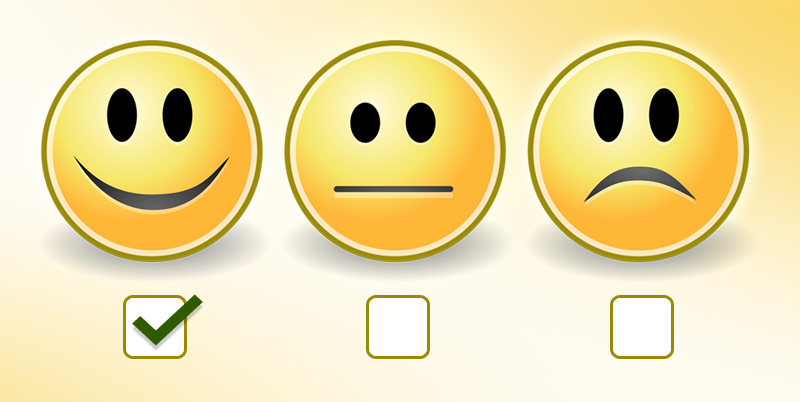
\includegraphics[scale = 0.15]{pics/sent.png}
        \end{figure}

  \item Las soluciones más avanzadas emplean modelos de aprendizaje automático \textbf{supervisado}, entrenados con ejemplos \textbf{anotados manualmente} \cite{Mohammad2013}.
\end{itemize}


\begin{figure}[h]
        	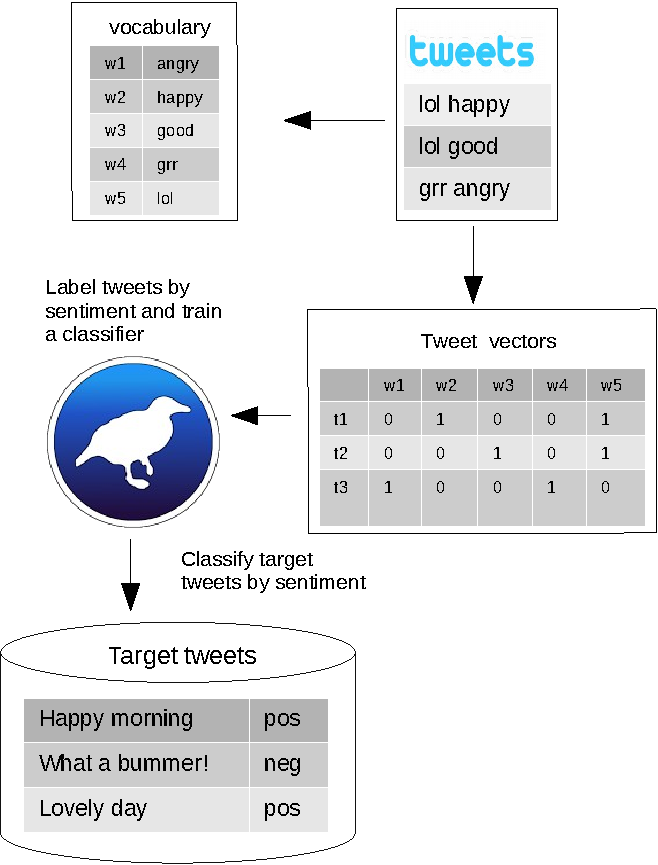
\includegraphics[scale = 0.5]{pics/bagOfwordsClassification.pdf}
        \end{figure}


\begin{itemize}


\item Idea: Encontrar un hiperplano que separe las clases con el margen máximo (mayor separación).

     \begin{figure}[h]
        	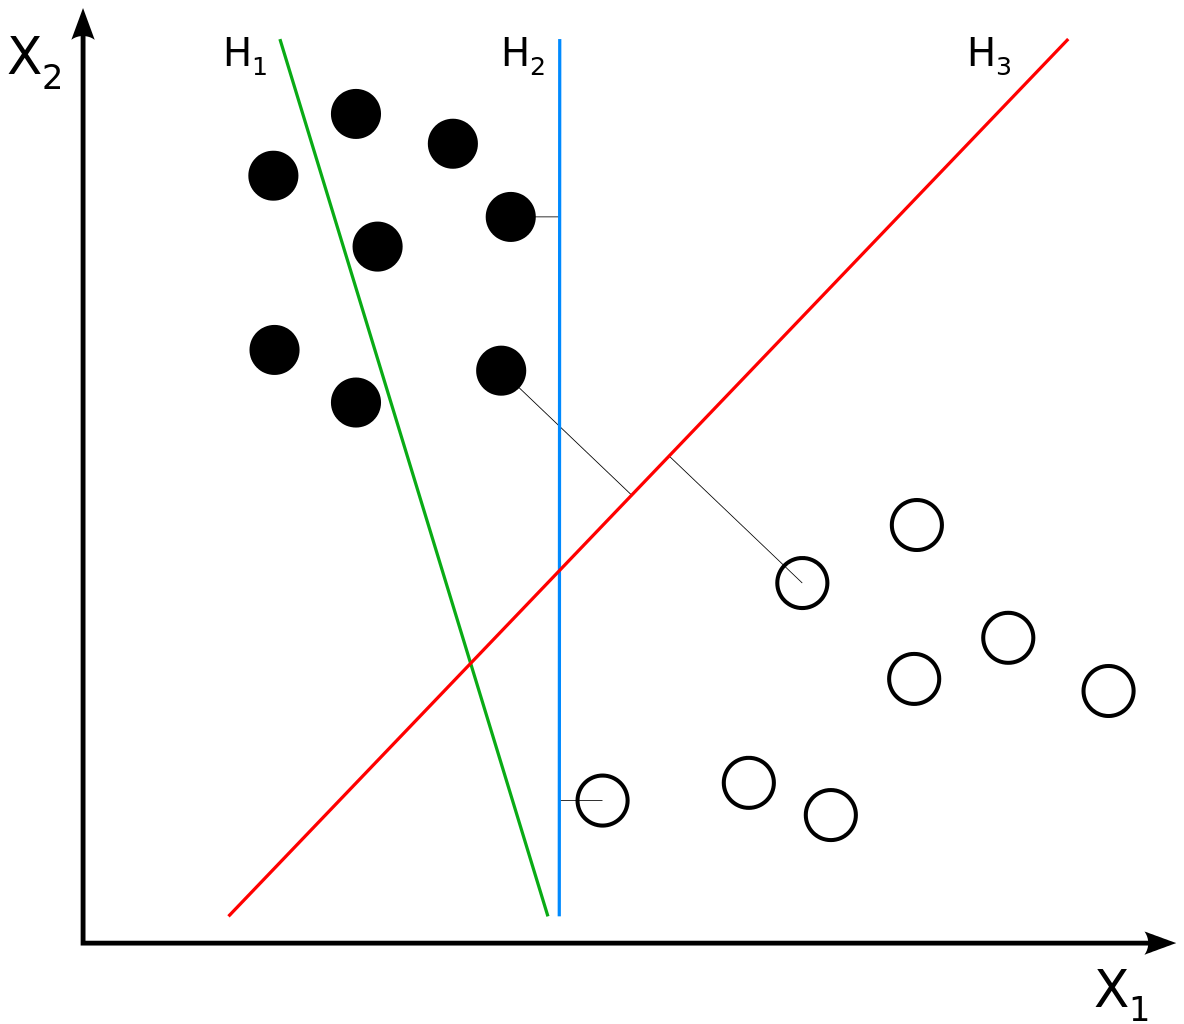
\includegraphics[scale = 0.15]{pics/SVM.png}
        \end{figure}

\item $H_3$ separa las clases con el margen máximo.

\end{itemize}


\subsection{Lingüística y Procesamiento del Lenguaje Natural (PNL)}

El conocimiento de las estructuras lingüísticas es fundamental para el diseño de características y el análisis de errores en el Procesamiento del Lenguaje Natural (PNL). Los enfoques de aprendizaje automático en PNL se basan en características que describen y generalizan las instancias de uso del lenguaje. El conocimiento lingüístico orienta la selección y el diseño de estas características, ayudando al algoritmo de aprendizaje automático a encontrar correlaciones entre el uso del lenguaje y las etiquetas objetivo \cite{bender2013linguistic}.

\begin{itemize}
  \item El conocimiento de las estructuras lingüísticas es importante para el diseño de características y el análisis de errores en PNL \cite{bender2013linguistic}.
  \item Los enfoques de aprendizaje automático en PNL requieren características que puedan describir y generalizar el uso del lenguaje.
  \item El objetivo es guiar al algoritmo de aprendizaje automático para encontrar correlaciones entre el uso del lenguaje y el conjunto de etiquetas objetivo.
  \item El conocimiento sobre las estructuras lingüísticas puede influir en el diseño de características para los enfoques de aprendizaje automático en PNL.
\end{itemize}

El PNL plantea diversos desafíos, como los costos de anotación, las variaciones de dominio y la necesidad de actualizaciones continuas. La anotación manual requiere mucho trabajo y tiempo. Las variaciones de dominio implican aprender patrones diferentes para diferentes corpus de texto. Los modelos entrenados en un dominio pueden no funcionar bien en otro. Además, los modelos de PNL pueden volverse obsoletos a medida que el uso del lenguaje evoluciona con el tiempo.




\section{Desafíos en el Procesamiento del Lenguaje Natural (PNL)}

\begin{itemize}
   \item \textbf{Costos de Anotación}: la anotación manual es \textbf{laboriosa} y \textbf{consume mucho tiempo}.
   \item \textbf{Variaciones de Dominio}: el patrón que queremos aprender puede variar de un corpus a otro (por ejemplo, deportes, política).

   \item ¡Un modelo entrenado con datos anotados de un dominio no necesariamente funcionará en otro!
   \item Los modelos entrenados pueden quedar desactualizados con el tiempo (por ejemplo, nuevos hashtags).
\end{itemize}

\paragraph{Variación de Dominio en el Análisis de Sentimiento}
\begin{enumerate}
   \item Para mí, la cola era bastante \textcolor[rgb]{0.00,0.00,1.00}{\textbf{pequeña}} y solo tuve que esperar unos 20 minutos, ¡pero valió la pena! :D @raynwise
   \item Extraña espacialidad en Stuttgart. La habitación del hotel es tan \textcolor[rgb]{1.00,0.00,0.00}{\textbf{pequeña}} que apenas puedo moverme, pero los alrededores son inhumanamente vastos y largos bajo construcción.
\end{enumerate}

\paragraph{Superando los costos de anotación de datos}
Supervisión Distant:
\begin{itemize}
   \item Etiquetar automáticamente datos no etiquetados (\textbf{API de Twitter}) utilizando un método heurístico.
   \item \textbf{Enfoque de Anotación de Emoticonos (EAA)}: los tweets con emoticonos positivos \textcolor[rgb]{0.00,0.00,1.00}{\textbf{:)}} o negativos \textcolor[rgb]{1.00,0.00,0.00}{\textbf{:(}} se etiquetan según la polaridad indicada por el emoticono~\cite{Read2005}.
   \item El emoticono se \textbf{elimina} del contenido.
   \item Este enfoque también se ha ampliado utilizando hashtags como \#anger y emojis.
   \item No es trivial encontrar técnicas de supervisión distante para todo tipo de problemas de PNL.
\end{itemize}

\paragraph{Crowdsourcing}
\begin{itemize}
   \item Confiar en servicios como \textbf{Amazon Mechanical Turk} o \textbf{Crowdflower} para solicitar a la \textbf{multitud} que anote datos.
   \item Esto puede resultar costoso.
   \item Es difícil garantizar la calidad de las anotaciones.
\end{itemize}

\section{Estudio de caso: Clasificación de sentimientos en tweets}

\begin{itemize}
   \item En 2013, el taller de Evaluación Semántica (SemEval) organizó la tarea de "Análisis de sentimientos en Twitter" \cite{Semeval2013}.
   \item La tarea se dividió en dos sub-tareas: el nivel de expresión y el nivel del mensaje.
   \item Nivel de expresión: se centró en determinar la polaridad del sentimiento de un mensaje según una entidad marcada dentro de su contenido.
   \item Nivel del mensaje: se debía determinar la polaridad según el mensaje en general.
   \item Los organizadores lanzaron conjuntos de datos de entrenamiento y prueba para ambas tareas \cite{Semeval2013}.
\end{itemize}

\paragraph{El sistema NRC}
\begin{itemize}
   \item El equipo que logró el mejor rendimiento en ambas tareas, entre 44 equipos, fue el equipo \emph{NRC-Canada} \cite{Mohammad2013}.
   \item El equipo propuso un enfoque supervisado utilizando un clasificador SVM lineal con las siguientes características hechas a mano para representar los tweets:
   \begin{enumerate}
      \item N-gramas de palabras.
      \item N-gramas de caracteres.
      \item Etiquetas de partes del discurso.
      \item Agrupaciones de palabras entrenadas con el método de agrupamiento de Brown \cite{brown1992class}.
      \item El número de palabras alargadas (palabras con un carácter repetido más de dos veces).
      \item El número de palabras con todas las letras en mayúscula.
      \item La presencia de emoticonos positivos o negativos.
      \item El número de negaciones individuales.
      \item El número de secuencias contiguas de puntos, signos de interrogación y signos de exclamación.
      \item Características derivadas de lexicones de polaridad \cite{Mohammad2013}. Dos de estos lexicones se generaron utilizando el método PMI a partir de tweets anotados con hashtags y emoticonos.
   \end{enumerate}
\end{itemize}

\section{Ingeniería de características y Aprendizaje Profundo}

\begin{itemize}
   \item Hasta 2014, la mayoría de los sistemas de PNL de última generación se basaban en ingeniería de características + modelos de aprendizaje automático superficiales (por ejemplo, SVM, HMM).
   \item Diseñar las características de un sistema de PNL ganador requiere mucho conocimiento específico del dominio.
   \item El sistema NRC se construyó antes de que el aprendizaje profundo se hiciera popular en PNL.
   \item Por otro lado, los sistemas de Aprendizaje Profundo se basan en redes neuronales para aprender automáticamente buenas representaciones.
\end{itemize}

\paragraph{Ingeniería de características y Aprendizaje Profundo}

\begin{figure}[h]
   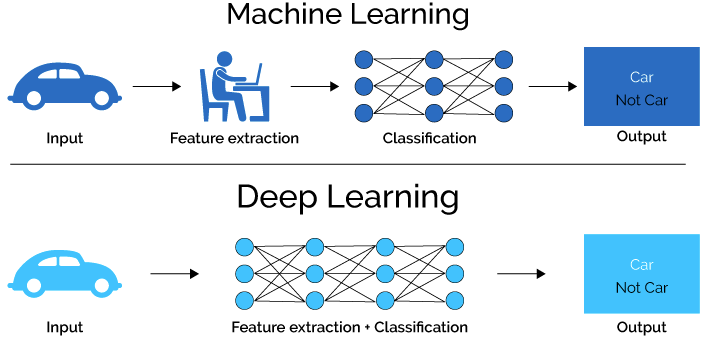
\includegraphics[scale = 0.25]{pics/MLvsDL.png}
\end{figure}

\begin{itemize}
   \item El Aprendizaje Profundo proporciona resultados de última generación en la mayoría de las tareas de PNL.
   \item Grandes cantidades de datos de entrenamiento y máquinas GPU

 multicore más rápidas son clave en el éxito del aprendizaje profundo.
   \item Las \textbf{redes neuronales} y las \textbf{incrustaciones de palabras} desempeñan un papel fundamental en los modelos modernos de PNL.

\end{itemize}

\paragraph{Aprendizaje Profundo y Conceptos Lingüísticos}
\begin{itemize}
   \item Si los modelos de aprendizaje profundo pueden aprender representaciones automáticamente, ¿siguen siendo útiles los conceptos lingüísticos (por ejemplo, sintaxis, morfología)?
   \item Algunos defensores del aprendizaje profundo argumentan que estas propiedades lingüísticas inferidas y diseñadas manualmente no son necesarias, y que la red neuronal aprenderá estas representaciones intermedias (o equivalentes o mejores) por sí misma \cite{goldberg2016primer}.
   \item Aún no hay un consenso definitivo al respecto.
   \item Goldberg cree que muchos de estos conceptos lingüísticos pueden ser inferidos por la red por sí misma si se le proporciona suficiente cantidad de datos.
   \item Sin embargo, en muchos otros casos no disponemos de suficientes datos de entrenamiento para la tarea que nos interesa, y en estos casos proporcionar a la red los conceptos generales más explícitos puede ser muy valioso.
\end{itemize}

\section{Historia}
El progreso de la PNL se puede dividir en tres oleadas principales: 1) racionalismo, 2) empirismo y 3) aprendizaje profundo \cite{deng2018deep}.
\begin{itemize}
   \item [1950 - 1990] Racionalismo: se enfocaba en diseñar reglas hechas a mano para incorporar conocimiento y mecanismos de razonamiento en sistemas de PNL inteligentes (por ejemplo, ELIZA para simular a un psicoterapeuta Rogeriano, MARGIE para estructurar información del mundo real en ontologías de conceptos).
   \item [1991 - 2009] Empirismo: se caracteriza por la explotación de corpora de datos y modelos de aprendizaje automático y estadísticos (superficiales) (por ejemplo, Naive Bayes, HMMs, modelos de traducción IBM).
   \item [2010 - ] Aprendizaje Profundo: la ingeniería de características (considerada como un cuello de botella) se reemplaza con el aprendizaje de representaciones y/o redes neuronales profundas (por ejemplo, \url{https://www.deepl.com/translator}). Un artículo muy influyente en esta revolución: \cite{collobert2011natural}.
\end{itemize}

\footnotetext{Las fechas son aproximadas.}

\section{Conclusiones}


En este capítulo, hemos explorado el desafío de entender y producir lenguaje utilizando computadoras. El aprendizaje automático supervisado es una de las principales técnicas utilizadas para abordar este desafío. Además, hemos discutido las propiedades desafiantes del lenguaje, como la discreción, la composicionalidad y la dispersión. Estos aspectos nos muestran la complejidad inherente al procesamiento del lenguaje natural y nos desafían a encontrar soluciones efectivas.



\bibliography{bio}
\bibliographystyle{apalike}

\end{document}
